%!TEX root = problems.tex
\printanswers

\begin{questions}

\question
	Consider the following graph.~\cite{biggs02}
  
  \begin{figure}[h]
  \centering
  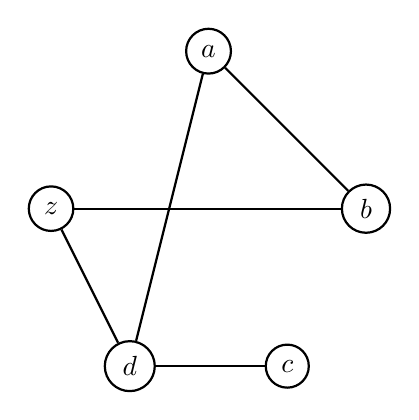
\begin{tikzpicture}[]
    \begin{scope}[every node/.style={circle,thick,draw}]
      \node (a) at (2,4) {$a$};
      \node (b) at (4,2) {$b$};
      \node (c) at (3,0) {$c$};
      \node (d) at (1,0) {$d$};
      \node (z) at (0,2) {$z$};
    \end{scope}
    \begin{scope}[every edge/.style={draw=black,thick}]
      \path (a) edge (b);
      \path (a) edge (d);
      \path (b) edge (z);
      \path (c) edge (d);
      \path (d) edge (z);
    \end{scope}
  \end{tikzpicture}
  \end{figure}
  
  \begin{parts}
    \part Determine the vertex set.
    \part Determine the edge set.
    \part Determine the adjacency list.
    \part For each of the vertices, determine the degree.
  \end{parts}
  
  \begin{solution}
    \begin{parts}
    	\part $ \{ a, b, c, d, z \} $.
  		\part $ \{ \{a, b\}, \{a, d\}, \{b, z\}, \{c, d\} \{d, z\} \} $.
		  \part \begin{tabular}{r|lll} a & b & d & \\ b & a & z & \\ c & d & & \\ d & a & c & z \\ z & b & d & \end{tabular}
		  \part $a: 2, b: 2, c: 1, d: 3, z:2$.
  	\end{parts}
  \end{solution}

\question
	Professor McBrain and his wife April give a party at which there are four other married couples.
	Some pairs of people shake hands when they meet, but naturally no couple shake hands with each other.
	At the end of the party the Professor asks everyone else how many people they have shaken hands with, and he receives nine different answers.~\cite{biggs02}
	
	\begin{parts}
		\part Draw a graph representing the handshakes exchanged at the party.
		\part How many people shook hands with April?
	\end{parts}
	
	\begin{solution}
		\begin{center}
  	 \begin{adjustbox}{max width=0.6\textwidth}
	  	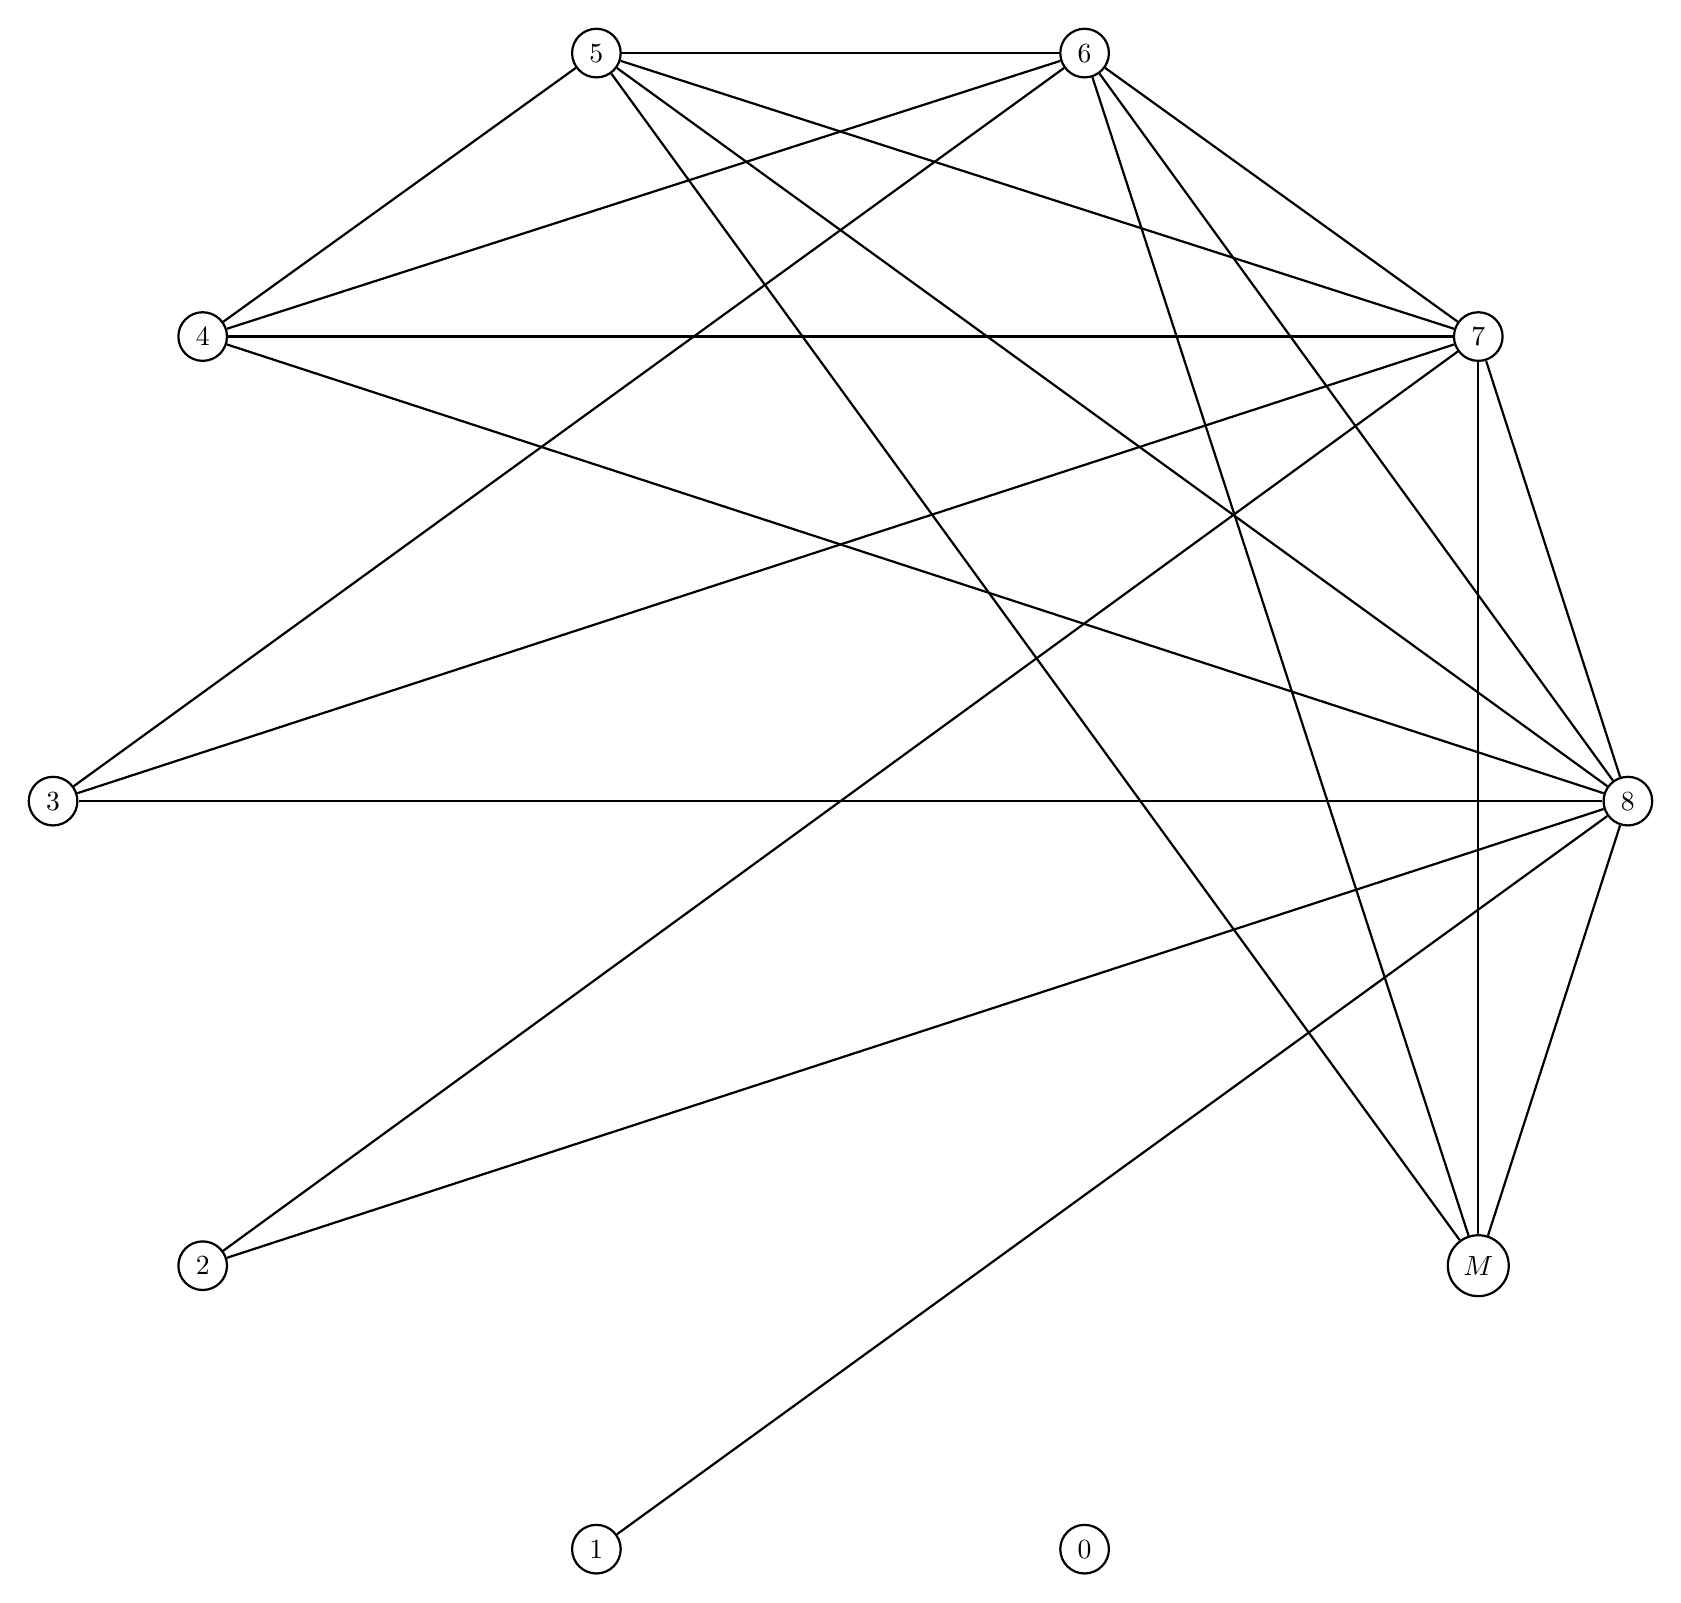
\begin{tikzpicture}
        \begin{scope}[every node/.style={circle,thick,draw}]
          \node (0) at (3.1,-9.5) {$0$};
          \node (1) at (-3.1,-9.5) {$1$};
          \node (2) at (-8.1,-5.9) {$2$};
          \node (3) at (-10.0,0) {$3$};
          \node (4) at (-8.1,5.9) {$4$};
          \node (5) at (-3.1,9.5) {$5$};
          \node (6) at (3.1,9.5) {$6$};
          \node (7) at (8.1,5.9) {$7$};
          \node (8) at (10.0,0) {$8$};
          \node (M) at (8.1,-5.9) {$M$};
          
        \end{scope}
        \begin{scope}[every edge/.style={draw=black,thick}]
          \path (8) edge (1);
          \path (8) edge (2);
          \path (8) edge (3);
          \path (8) edge (4);
          \path (8) edge (5);
          \path (8) edge (6);
          \path (8) edge (7);
          \path (8) edge (M);
          \path (7) edge (6);
          \path (7) edge (5);
          \path (7) edge (4);
          \path (7) edge (3);
          \path (7) edge (2);
          \path (7) edge (M);
          \path (6) edge (5);
          \path (6) edge (4);
          \path (6) edge (3);
          \path (6) edge (M);
          \path (5) edge (4);
          \path (5) edge (M);
        \end{scope}
  		\end{tikzpicture}
		\end{adjustbox}
		\end{center}

	
  	We construct a graph whose vertices are the people at the party, and there is an edge (x, y) whenever x and y shook hands.
  	Since there are nine people apart from Professor McBrain, and the maximum number of handshakes in which any one person can be involved is eight, it follows that the nine different answers received by the Professor must be 0, 1, 2, 3, 4, 5, 6, 7, 8.
  	We denote the vertices by these numbers and use M for McBrain himself.
  	So we have a pictorial representation.
  	Now, vertex 8 is joined to all the other vertices except one, which must therefore represent the spouse of 8.
  	This vertex must be 0, since it is certainly not joined to 8 (or any other vertex, for that matter).
  	Thus 8 and 0 are a married couple, and 8 is joined to 1, 2, ..., 7 and M.
  	In particular 1 is joined to 8 and this is the only edge from 1.
  	Hence vertex 7 is not joined to 0 and 1 (only), and the spouse of 7 must be 1, since 0 is married to 8.
  	Continuing in the same way, we see that 6 and 2, and 5 and 3 are married couples.
  	It follows that M and 4 are married, so vertex 4 represents April, who shook hands with four people.
  \end{solution}

\question
  Three houses A, B, C each has to be connected to the gas, water and electricity supplies: G, W, E.
  Write down the adjacency list for the graph which represents this problem, and construct a pictorial representation of it.
  Can you find a picture in which the lines representing the edges do not cross?~\cite{biggs02}
	\begin{solution}
		
		Adjacency list:
		\begin{center}
  		\begin{tabular}{r|lll}
  			A & G & E & W \\
  			B & G & E & W \\
  			C & G & E & W \\
  			G & A & B & C \\
  			E & A & B & C \\
  			W & A & B & C
  		\end{tabular}
		\end{center}
		
		Pictorial representation:
		\begin{center}
  	 \begin{adjustbox}{max width=0.6\textwidth}
	  	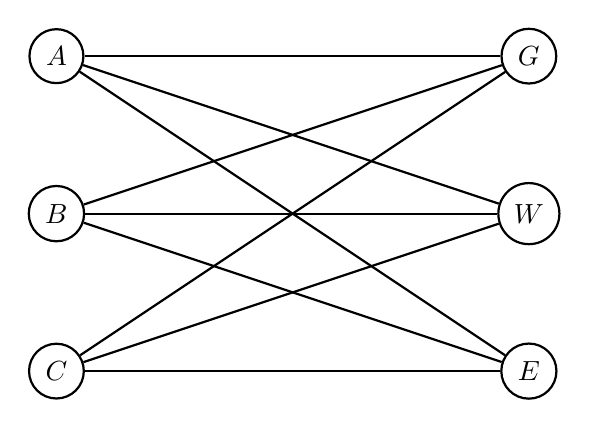
\begin{tikzpicture}
        \begin{scope}[every node/.style={circle,thick,draw}]
          \node (A) at (0,4) {$A$};
          \node (B) at (0,2) {$B$};
          \node (C) at (0,0) {$C$};
          \node (G) at (6,4) {$G$};
          \node (W) at (6,2) {$W$};
          \node (E) at (6,0) {$E$};
          
        \end{scope}
        \begin{scope}[every edge/.style={draw=black,thick}]
          \path (A) edge (G);
          \path (B) edge (W);
          \path (C) edge (E);
          \path (A) edge (W);
          \path (B) edge (E);
          \path (C) edge (G);
          \path (A) edge (E);
          \path (B) edge (G);
          \path (C) edge (W);
        \end{scope}
  		\end{tikzpicture}
			\end{adjustbox}
		\end{center}
		It's impossible to draw the graph without some edges crossing.
		This will be proven in later lectures.
	\end{solution}
	


\question
  The pathways in a formal garden are to be laid out in the form of a wheel graph $W_n$ whose vertex set is $V = \{0,1,2,\ldots,n\}$ and whose edges are:
  \begin{align*}
  	&\{0,1\}, \{0,2\}, \ldots, \{0,n\}, \\
  	&\{1,2\}, \{2,3\}, \ldots, \{n-1,n\}, \{n,1\}
  \end{align*}
  Describe a route around the pathways which starts and ends at vertex 0 and visits every vertex once only.~\cite{biggs02}

	\begin{solution}
	
		Say, for n = 6, we could draw the graph this way:
		\begin{center}
  	 \begin{adjustbox}{max width=0.6\textwidth}
	  	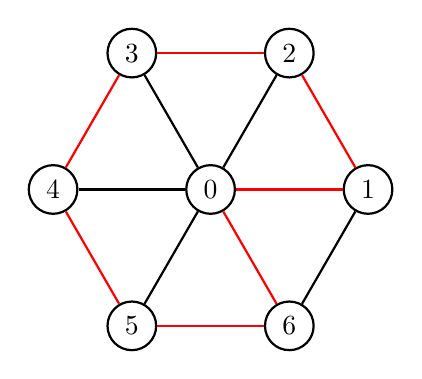
\begin{tikzpicture}
        \begin{scope}[every node/.style={circle,thick,draw}]
          \node (0) at (0,0) {$0$};
          \node (1) at (2,0) {$1$};
          \node (2) at (1,1.732) {$2$};
          \node (3) at (-1,1.732) {$3$};
          \node (4) at (-2,0) {$4$};
          \node (5) at (-1,-1.732) {$5$};
          \node (6) at (1,-1.732) {$6$};

          
        \end{scope}
        \begin{scope}[every edge/.style={draw=black,thick}]
          \path (0) edge [red] (1);
          \path (0) edge (2);
          \path (0) edge (3);
          \path (0) edge (4);
          \path (0) edge (5);
          \path (0) edge [red] (6);
          \path (1) edge [red] (2);
          \path (2) edge [red] (3);
          \path (3) edge [red] (4);
          \path (4) edge [red] (5);
          \path (5) edge [red] (6);
          \path (6) edge (1);
        \end{scope}
  		\end{tikzpicture}
			\end{adjustbox}
		\end{center}
		
		One such path is given in red.
	\end{solution}

\question
  For each positive integer $n$ we define the complete graph $K_n$ to be the graph with n vertices in which each pair of vertices is adjacent.~\cite{biggs02}
  \begin{parts}
  	\part How many edges has $K_n$?
  	\part For which values of $n$ can you find a pictorial representation of $K_n$ with the property that the lines representing the edges do not cross?
  \end{parts}

	\begin{solution}
		Every edge is connected to every other.
		Every edge looks like $\{a,b\}$ where $a$ and $b$ are vertices.
		There are $n$ choices for $a$, and then $n-1$ for $b$.
		So the total number of edges seems to be $n(n-1)$.
		However, we've now counted the edge $\{a,b\}$ twice -- once as $\{a,b\}$ and once as $\{b,a\}$.
		So the actual number of edges in $K_n$ is:
		$$ \frac{n(n-1)}{2}$$
	\end{solution}

\question
  A 3-cycle in a graph is a set of three mutually adjacent vertices.
  Construct a graph with five vertices and six edges which contains no 3-cycles.~\cite{biggs02}

	\begin{solution}
		There are lots of possibilities. Here's one:
		\begin{center}
  	 \begin{adjustbox}{max width=0.6\textwidth}
	  	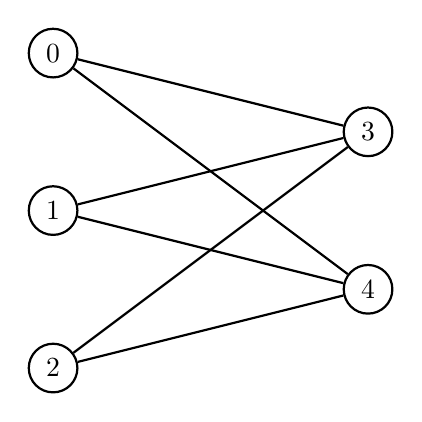
\begin{tikzpicture}
        \begin{scope}[every node/.style={circle,thick,draw}]
          \node (1) at (0,4) {$0$};
          \node (2) at (0,2) {$1$};
          \node (3) at (0,0) {$2$};
          \node (4) at (4,3) {$3$};
          \node (5) at (4,1) {$4$};
          
        \end{scope}
        \begin{scope}[every edge/.style={draw=black,thick}]
          \path (1) edge (4);
          \path (2) edge (4);
          \path (3) edge (4);
          \path (1) edge (5);
          \path (2) edge (5);
          \path (3) edge (5);
        \end{scope}
  		\end{tikzpicture}
			\end{adjustbox}
		\end{center}

	\end{solution}

\question
  Consider the following two graphs $G_1 = (V_1,E_1)$ and $G_2 = (V_2,E_2)$ where:
  \begin{align*}
    V_1 &= \{a,b,c,d\} \\
    E_1 &= \{\{a,b\},\{b,c\},\{b,d\},\{c,d\}\}\\
    V_2 &= \{1,2,3,4\} \\
    E_2 &= \{\{1,2\},\{1,3\},\{1,4\},\{3,4\}\}
  \end{align*}

  \begin{parts}
    \part Draw a picture of each of the graphs.
    \begin{solution}
      \begin{center}
        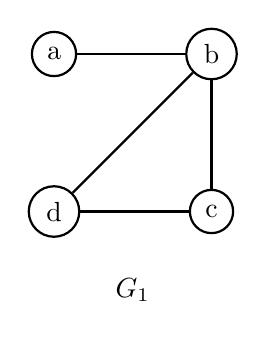
\begin{tikzpicture}
          \begin{scope}[every node/.style={circle,thick,draw}]
            \node (a) at (0,2) {a};
            \node (b) at (2,2) {b};
            \node (c) at (2,0) {c};
            \node (d) at (0,0) {d};
          \end{scope}
          \begin{scope}[every edge/.style={draw=black,thick}]
            \path (a) edge (b);
            \path (b) edge (c);
            \path (b) edge (d);
            \path (c) edge (d);
          \end{scope}
          \node () at (1,-1) {$G_1$};
        \end{tikzpicture}
        \hspace{1.5cm}
        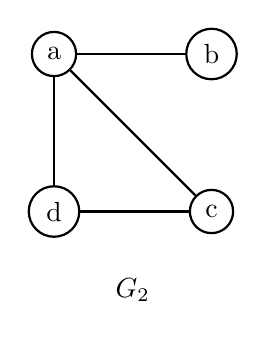
\begin{tikzpicture}
          \begin{scope}[every node/.style={circle,thick,draw}]
            \node (1) at (0,2) {a};
            \node (2) at (2,2) {b};
            \node (3) at (2,0) {c};
            \node (4) at (0,0) {d};
          \end{scope}
          \begin{scope}[every edge/.style={draw=black,thick}]
            \path (1) edge (2);
            \path (1) edge (3);
            \path (1) edge (4);
            \path (3) edge (4);
          \end{scope}
          \node () at (1,-1) {$G_2$};
          \end{tikzpicture}
        \end{center}
    \end{solution}
    \part Determine a bijection between the vertex sets that preserves the edges.
    \begin{solution}
       There are lots of bijections between $V_1$ and $V_2$.
       However, not all of them preserve the edges.
       For instance the following bijection \textbf{will not} work:
       \begin{align*}
         f(a) = 1; f(b) = 2; f(c) = 3; f(d) = 4
       \end{align*}
       When we apply f to the edges in this case:
       \begin{align*}
         f(E_1) &= \{\{f(a),f(b)\},\{f(b),f(c)\},\{f(b),f(d)\},\{f(c),f(d)\}\} \\
                &= \{\{1,2\},\{2,3\},\{2,4\},\{3,4\}\} \\
                &\neq E_2.
       \end{align*}
       
       Here's an answer to the question -- a bijection that will work:
      \begin{align*}
        f(a) = 2; f(b) = 1; f(c) = 3; f(d) = 4
      \end{align*}
      Then:
      \begin{align*}
        f(E_1) &= \{\{f(a),f(b)\},\{f(b),f(c)\},\{f(b),f(d)\},\{f(c),f(d)\}\} \\
               &= \{\{2,1\},\{1,3\},\{1,4\},\{3,4\}\} \\
               &= E_2.
      \end{align*}
      Remember that sets don't have order, so $\{1,2\} = \{2,1\}$.
        
    \end{solution}
  \end{parts}

\question
  Determine if the following two graphs are isomorphic.

  \begin{center}
    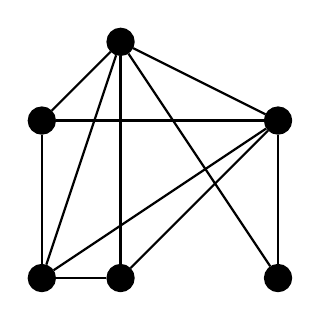
\begin{tikzpicture}
      \begin{scope}[every node/.style={circle,thick,draw,fill}]
        \node (a) at (0,1) {};
        \node (b) at (0,4) {};
        \node (c) at (2,1) {};
        \node (d) at (2,3) {};
        \node (e) at (-1,1) {};
        \node (f) at (-1,3) {};
      \end{scope}
      \begin{scope}[every edge/.style={draw=black,thick}]
        \path (a) edge (b);
        \path (a) edge (d);
        \path (a) edge (e);
        \path (b) edge (c);
        \path (b) edge (d);
        \path (b) edge (e);
        \path (b) edge (f);
        \path (c) edge (d);
        \path (d) edge (e);       
        \path (d) edge (f);
        \path (e) edge (f);
      \end{scope}
    \end{tikzpicture}
    \hspace{1.5cm}
    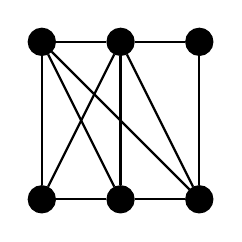
\begin{tikzpicture}
      \begin{scope}[every node/.style={circle,thick,draw,fill}]
        \node (a) at (0,0) {};
        \node (b) at (0,2) {};
        \node (c) at (1,0) {};
        \node (d) at (1,2) {};
        \node (e) at (2,0) {};
        \node (f) at (2,2) {};
      \end{scope}
      \begin{scope}[every edge/.style={draw=black,thick}]
          \path (a) edge (b);
          \path (a) edge (c);
          \path (a) edge (d);
          \path (b) edge (c);
          \path (b) edge (d);
          \path (b) edge (e);
          \path (b) edge (d);
          \path (c) edge (d);
          \path (c) edge (e);
          \path (d) edge (e);         
          \path (e) edge (f);
          \path (d) edge (f);
      \end{scope}
    \end{tikzpicture}
  \end{center}

  \begin{solution}
    The first step here is to label the vertices and give the graphs names.
    Then we can work on finding a bijection.
    \begin{center}
      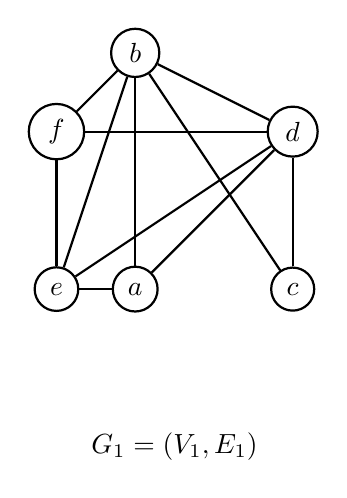
\begin{tikzpicture}
        \begin{scope}[every node/.style={circle,thick,draw}]
          \node (a) at (0,1) {$a$};
          \node (b) at (0,4) {$b$};
          \node (c) at (2,1) {$c$};
          \node (d) at (2,3) {$d$};
          \node (e) at (-1,1) {$e$};
          \node (f) at (-1,3) {$f$};
        \end{scope}
      \begin{scope}[every edge/.style={draw=black,thick}]
        \path (a) edge (b);
        \path (a) edge (d);
        \path (a) edge (e);
        \path (b) edge (c);
        \path (b) edge (d);
        \path (b) edge (e);
        \path (b) edge (f);
        \path (c) edge (d);
        \path (d) edge (e);       
        \path (d) edge (f);
        \path (e) edge (f);
      \end{scope}
      \node () at (0.5,-1) {$G_1 = (V_1,E_1)$};
      \end{tikzpicture}
      \hspace{1.5cm}
      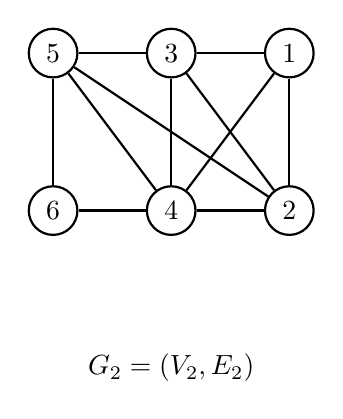
\begin{tikzpicture}
        \begin{scope}[every node/.style={circle,thick,draw}]
          \node (a) at (2,3) {1};
          \node (b) at (2,1) {2};
          \node (c) at (0.5,3) {3};
          \node (d) at (0.5,1) {4};
          \node (e) at (-1,3) {5};
          \node (f) at (-1,1) {6};
        \end{scope}
        \begin{scope}[every edge/.style={draw=black,thick}]
          \path (a) edge (b);
          \path (a) edge (c);
          \path (a) edge (d);
          \path (b) edge (c);
          \path (b) edge (d);
          \path (b) edge (e);
          \path (b) edge (d);
          \path (c) edge (d);
          \path (c) edge (e);
          \path (d) edge (e);         
          \path (e) edge (f);
          \path (d) edge (f);
        \end{scope}
      \node () at (0.5,-1) {$G_2 = (V_2,E_2)$};
      \end{tikzpicture}
    \end{center}

    It's worth checking first if there are the same number of vertices and edges in the two graphs.
    If not, they can't be isomorphic.
    They both have $6$ vertices, and $11$ edges.
    
    Next let's check that we have the same number of vertices in each graph with a given degree.
    If we don't, they can't be isomorphic.
    The degrees are:
    \begin{align*}
      &G_1& \qquad &G_2& \\
      &\delta(a) = 2& &\delta(1) = 3& \\
      &\delta(b) = 5& &\delta(2) = 4& \\
      &\delta(c) = 2& &\delta(3) = 4& \\
      &\delta(d) = 5& &\delta(4) = 5& \\
      &\delta(e) = 4& &\delta(5) = 4& \\
      &\delta(f) = 3& &\delta(6) = 2&
    \end{align*}
    So we can see that the graphs cannot be isomorphic, since every vertex in $G_1$ would have to map to a vertex of equal degree in $G_2$.
    This isn't possible since, for instance, we have two vertices of degree $2$ in $G_1$, and only one in $G_2$.
  \end{solution}

\question
  Determine three different isomorphisms between the following two graphs:
  \begin{center}
    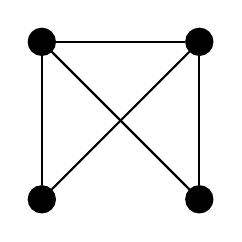
\begin{tikzpicture}
      \begin{scope}[every node/.style={circle,thick,draw,fill}]
        \node (a) at (0,0) {};
        \node (b) at (0,2) {};
        \node (c) at (2,0) {};
        \node (d) at (2,2) {};
      \end{scope}
      \begin{scope}[every edge/.style={draw=black,thick}]
        \path (a) edge (b);
        \path (a) edge (d);
        \path (b) edge (c);
        \path (b) edge (d);
        \path (c) edge (d);
      \end{scope}
    \end{tikzpicture}
    \hspace{1.5cm}
    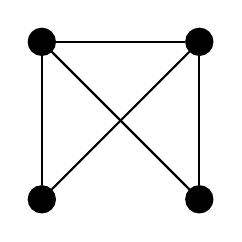
\begin{tikzpicture}
      \begin{scope}[every node/.style={circle,thick,draw,fill}]
        \node (a) at (0,0) {};
        \node (b) at (0,2) {};
        \node (c) at (2,0) {};
        \node (d) at (2,2) {};
      \end{scope}
      \begin{scope}[every edge/.style={draw=black,thick}]
        \path (a) edge (b);
        \path (a) edge (d);
        \path (b) edge (c);
        \path (b) edge (d);
        \path (c) edge (d);
      \end{scope}
    \end{tikzpicture}
  \end{center}

  \begin{solution}
    Again, label the vertices.
      \begin{center}
        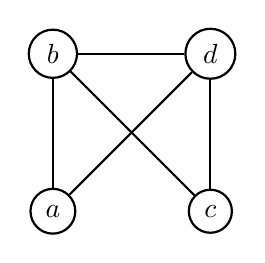
\begin{tikzpicture}
        \begin{scope}[every node/.style={circle,thick,draw}]
        \node (a) at (0,0) {$a$};
        \node (b) at (0,2) {$b$};
        \node (c) at (2,0) {$c$};
        \node (d) at (2,2) {$d$};
        \end{scope}
        \begin{scope}[every edge/.style={draw=black,thick}]
        \path (a) edge (b);
        \path (a) edge (d);
        \path (b) edge (c);
        \path (b) edge (d);
        \path (c) edge (d);
        \end{scope}
        \end{tikzpicture}
        \hspace{1.5cm}
        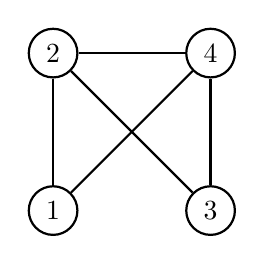
\begin{tikzpicture}
        \begin{scope}[every node/.style={circle,thick,draw}]
        \node (a) at (0,0) {1};
        \node (b) at (0,2) {2};
        \node (c) at (2,0) {3};
        \node (d) at (2,2) {4};
        \end{scope}
        \begin{scope}[every edge/.style={draw=black,thick}]
        \path (a) edge (b);
        \path (a) edge (d);
        \path (b) edge (c);
        \path (b) edge (d);
        \path (c) edge (d);
        \end{scope}
        \end{tikzpicture}
      \end{center}
      Here are three isomorphisms that work:
      \begin{align*}
      &\textbf{\textrm{Ismorphism 1:}} \qquad f(a) = 1; f(b) = 2; f(c) = 3; f(d) = 4& \\
      &\textbf{\textrm{Ismorphism 2:}} \qquad g(a) = 3; g(b) = 2; g(c) = 1; g(d) = 4& \\
      &\textbf{\textrm{Ismorphism 3:}} \qquad h(a) = 1; h(b) = 4; h(c) = 3; h(d) = 2&
      \end{align*}
      You should check that these preserve the edges.
      There are more isomorphisms, and there are bijections that are not isomorphisms.
      You could easily list them all.
      In an exam, you should always show that the isomorphism preserves the edges by mapping all of the edges one by one.
  \end{solution}


\question
  Prove that these graphs are not isomorphic~\cite{biggs02}:
  \begin{center}
    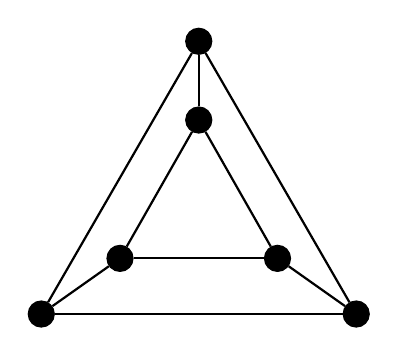
\begin{tikzpicture}
      \begin{scope}[every node/.style={circle,draw,fill}]
        \node (a) at (0,0) {};
        \node (b) at (4,0) {};
        \node (c) at (2,3.464) {};
        \node (d) at (1,0.707) {};
        \node (e) at (3,0.707) {};
        \node (f) at (2,2.464) {};
      \end{scope}
      \begin{scope}[every edge/.style={draw=black,thick}]
        \path (a) edge (b);
        \path (a) edge (c);
        \path (c) edge (b);
        \path (d) edge (e);
        \path (d) edge (f);
        \path (e) edge (f);
        \path (b) edge (e);
        \path (c) edge (f);
        \path (a) edge (d);
      \end{scope}
    \end{tikzpicture}
    \hspace{1.5cm}
    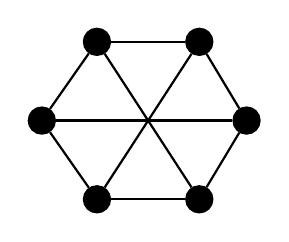
\begin{tikzpicture}
      \begin{scope}[every node/.style={circle,thick,draw,fill}]
        \node (a) at (0,1) {};
        \node (b) at (0.7,0) {};
        \node (c) at (2,0) {};
        \node (d) at (2.6,1) {};
        \node (e) at (2,2) {};
        \node (f) at (0.7,2) {};
      \end{scope}
      \begin{scope}[every edge/.style={draw=black,thick}]
        \path (a) edge (b);
        \path (b) edge (c);
        \path (c) edge (d);
        \path (d) edge (e);
        \path (e) edge (f);
        \path (f) edge (a);
        \path (a) edge (d);
        \path (b) edge (e);
        \path (c) edge (f);
      \end{scope}
    \end{tikzpicture}
  \end{center}

\begin{solution}
  The graphs both have six vertices of degree three, so we can't rule out an isomorphism based on degrees of vertices.
  However, the graph on the left has two 3-cycles.
  The one on the right has none.
  Isomorphic graphs have the same number of $3$-cycles, or $n$-cycles for any $n$ for that matter.
  You should convince yourself of that fact.
\end{solution}

\question
  Find an isomorphism between the graphs defined by the following adjacency lists~\cite{biggs02}.
  \begin{center}
    \begin{tabular}{cccccccccc}
      a & b & c & d & e & f & g & h & i & j \\
      \hline
      b & a & b & c & d & a & b & c & d & e \\
      e & c & d & e & a & h & i & j & f & g \\
      f & g & h & i & j & i & j & f & g & h 
    \end{tabular}
    \hspace{1cm}
    \begin{tabular}{cccccccccc}
      0 & 1 & 2 & 3 & 4 & 5 & 6 & 7 & 8 & 9 \\
      \hline
      1 & 2 & 3 & 4 & 5 & 0 & 1 & 0 & 2 & 6 \\
      5 & 0 & 1 & 2 & 3 & 4 & 4 & 3 & 5 & 7 \\
      7 & 6 & 8 & 7 & 6 & 8 & 9 & 9 & 9 & 8 
    \end{tabular}
  \end{center}

\begin{solution}
  There are lots, we just have to find one.
  We can do this by trial and error -- try a bijection between the vertices of the first graph and the second graph and see if it works.
  Then adapt it if it doesn't work.
  
  One that will work is:
  \begin{align*}
  &f(\textrm{a}) = 4; f(\textrm{b}) = 3; f(\textrm{c}) = 2; f(\textrm{d}) = 1; f(\textrm{e}) = 6; \\
  &f(\textrm{f}) = 5; f(\textrm{g}) = 7; f(\textrm{h}) = 8; f(\textrm{i}) = 0; f(\textrm{j}) = 9;
  \end{align*}
  
  The point of this question is to highlight how hard finding an isomorphism generally is.
\end{solution}


\question
  Show that the graph given by the following adjacency list~\cite{biggs02}:
  \begin{center}
    \begin{tabular}{cccccccc}
      000 & 001 & 010 & 011 & 100 & 101 & 110 & 111 \\
      \hline
      001 & 000 & 011 & 010 & 000 & 100 & 111 & 110 \\
      010 & 011 & 000 & 001 & 110 & 111 & 100 & 101 \\
      100 & 101 & 110 & 111 & 101 & 001 & 010 & 011
    \end{tabular}
  \end{center}
  is isomorphic to the following graph:
  \begin{center} 
    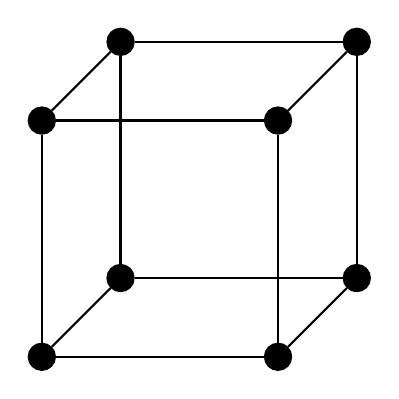
\begin{tikzpicture}
      \begin{scope}[every node/.style={circle,thick,draw,fill}]
        \node (a) at (0,0) {};
        \node (b) at (0,3) {};
        \node (d) at (3,0) {};
        \node (c) at (3,3) {};
        \node (e) at (1,1) {};
        \node (f) at (1,4) {};
        \node (h) at (4,1) {};
        \node (g) at (4,4) {};
      \end{scope}
      \begin{scope}[every edge/.style={draw=black,thick}]
        \path (a) edge (b);
        \path (b) edge (c);
        \path (c) edge (d);
        \path (d) edge (a);
        \path (e) edge (f);
        \path (f) edge (g);
        \path (g) edge (h);
        \path (h) edge (e);
        \path (a) edge (e);
        \path (b) edge (f);
        \path (c) edge (g);
        \path (d) edge (h);
      \end{scope}
    \end{tikzpicture}
  \end{center}


\begin{solution}
  Label the graph as follows:
  
    \begin{center} 
      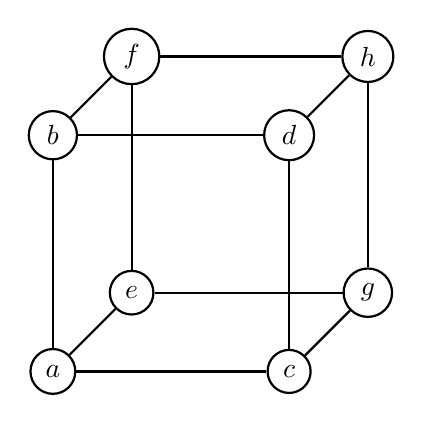
\begin{tikzpicture}
      \begin{scope}[every node/.style={circle,thick,draw}]
      \node (a) at (0,0) {$a$};
      \node (b) at (0,3) {$b$};
      \node (d) at (3,0) {$c$};
      \node (c) at (3,3) {$d$};
      \node (e) at (1,1) {$e$};
      \node (f) at (1,4) {$f$};
      \node (h) at (4,1) {$g$};
      \node (g) at (4,4) {$h$};
      \end{scope}
      \begin{scope}[every edge/.style={draw=black,thick}]
      \path (a) edge (b);
      \path (b) edge (c);
      \path (c) edge (d);
      \path (d) edge (a);
      \path (e) edge (f);
      \path (f) edge (g);
      \path (g) edge (h);
      \path (h) edge (e);
      \path (a) edge (e);
      \path (b) edge (f);
      \path (c) edge (g);
      \path (d) edge (h);
      \end{scope}
      \end{tikzpicture}
    \end{center}
    
    In the adjacency list, every vertex is adjacent to, and only to, the vertices that differ from it in exactly one digit.
    Treat the three digits as coordinates in 3D space, so 101 is 1 in the $x$ direction, 0 in the $y$ direction and $1$ in the $z$ direction.
    Then the following bijection is an isomorphism:
    \begin{align*}
      &f(\textrm{a}) = 000; f(\textrm{b}) = 010; f(\textrm{c}) = 100; f(\textrm{d}) = 110; \\
      &f(\textrm{e}) = 001; f(\textrm{f}) = 011; f(\textrm{g}) = 101; f(\textrm{h}) = 111;
    \end{align*}
    There are many other isomorphisms.
    Try, for instance, rotating the cube using one of its symmetries.
\end{solution}




\end{questions}
